%----------------------------------------------------------
\def\notedate{2021.10.05}
\def\currentauthor{Ершов В. (РК6-72Б)}
%----------------------------------------------------------
\notestatement{rndhpcedt}{Обзор языка описания графов DOT}

Язык описания графов DOT предоставляется пакетом утилит Graphviz (Graph Visualization Software). Пакет состоит из набора утилит командной строки и программ с графическим интерфейсом, способных обрабатывать файлы на языке DOT, а также из виджетов и библиотек, облегчающих создание графов и программ для построения графов. Более подробно будет рассмотрена утилита dot.

\begin{remark}
dot -- программный инструмент для создания многоуровневого графа с возможностью вывода изображения полученного графа в различных форматах (PNG, PDF, PostScript, SVG и др.).
\end{remark}

Установка graphviz:

\quad Linux: \lstinline$sudo apt install graphviz$

\quad MacOS: \lstinline$brew install graphviz$


Вызов всех программ Graphviz осуществляется через командную строку, в процессе ознакомления с языком использовалась следующая команда:

\quad\lstinline$dot -Tpng <pathToDotFile> -o <imageName>$

В результате выполнения этой команды будет создано изображение графа в формате png.

Пример описания простого графа на языке DOT представлен далее.

\begin{minipage}{0.2\textwidth}
		\begin{verbatim}
				digraph G {
				    a -> b;
				    a -> d -> c;
				    d -> e;
				}
		\end{verbatim}
	\end{minipage}
	\hfill
	\begin{minipage}{0.75\textwidth}
%	\begin{figure}[!ht]
	\center{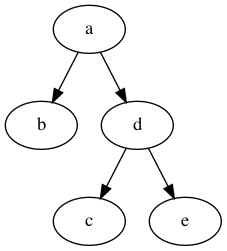
\includegraphics[width=0.3\textwidth]{ResearchNotes/rndhpc_not_edt_2021_10_05/image4.png}}
%	\caption{Пример визуализации DOT}\label{fig:image4}
%	\end{figure}
	\end{minipage}

Более подробная информация с примерами представлена в обзоре литературы, который размещён по следующему адресу:

\textsf{01 - Курсовые проекты/2021-2022 - Разработка web-ориентированного редактора графовых моделей /0 - Обзор литературы/	}

%----------------------------------------------------------
% Атрибуты задачи
\noteattributes{}
%----------------------------------------------------------